\documentclass{ltjarticle}
\usepackage{geometry}
\usepackage[dvipdfmx]{graphicx}
\usepackage[colorlinks=true, allcolors=blue] {hyperref}
\usepackage{amsmath}
\usepackage{mathtools}
% ページの余白を1.25インチにする
\geometry{
    left=1.25truein,
    right=1.25truein,
    top=1.25truein,
    bottom=1.25truein,
}

\begin{document}
\begin{titlepage}
    \begin{center}
        {\Large 令和5年}
        \vspace{10truept}

        {\Large 修士論文草稿}
        \vspace*{180truept}

        {\Huge タイトル} 
        \vspace{160truept}

        {\Large 指導教員:相馬 隆郎}
        \vspace{30truept}

        {\Large 東京都立大学大学院}
        \vspace{10truept}

        {\Large 電子情報システム工学域}
        \vspace{30truept}

        {\Large 学修番号:22861651}
        \vspace{10truept}
        
        {\Large 氏名:西原涼介}
    \end{center}
\end{titlepage}
\noindent
{\LARGE 論文要旨}
\vspace{20truept}

ここから論文要旨

% 目次
\newpage
\tableofcontents
\clearpage

\part{はじめに}
\vspace{10truept}
\section{研究背景}
近年, Amazonや楽天市場などの大手ECサイトをはじめ、数多くのECサイトが普及し,  その利用者も急増して
いる. そして, 商品を購入する際にECサイトのレビューを参考にしている利用者の割合は約70\%と言われていて, そ
の中でもレビューの信頼性を重要視している人が多いことが明らかになっている. また, 多くの企業にとって, ECサイトの
レビューからユーザーの嗜好や意見を分析し,マーケティングに活用することが重要な課題となっている.そのため,
ECサイトのレビューの信頼性や参考になるかどうかを評価する評判分析や口コミ分析, レビューを様々なトピックに分類する文書分類に関する
研究が多く行われている. 例えば, 関連研究の項で詳しく紹介する「機械学習を用いた自然言語処理による商品レビューの評価」[1]では, Amazonの商品レビュー
を機械学習を用いて参考になる順に並びかえるシステムの構築, 及びその評価に関する研究を行っている。
また近年では, 従来のECサイトや商品のWebページ以外にも, YouTubeのような
動画投稿サイトやX(旧Twitter)やInstagramなどのSNSで自社製品・サービスの宣伝を行う企業が増えてきている. 
それにつれて, 商品を購入する際にSNSやYouTube上でその商品を宣伝している投稿を参考にしている人も増加している. 
そのため, SNSやYouTube上の広告に対するユーザーのコメントも, 他のユーザーが商品の購入を検討する際の重要な判断
材料になり得ると考えられる. つまり, SNSやYouTube上での商品の宣伝に対するコメントは, ECサイトのレビュー
と同等の機能を持ち, その信頼性や参考になるかどうかが重要になるため, 
評判分析や文書分類の研究の対象になると考えられる. ここで, SNSやYouTubeは商品レビューのページとは異なり, 
誰でも気軽にコメントを投稿できたり, その投稿内容も自由という特性上, 商品やサービスに関係ないコメントが
多数存在する.

そこで, 本研究では分析対象をYouTube上で自社製品やサービスを宣伝している動画に対するユーザーのコメントとし, 
トピックモデルの一種であるBiterm Topic Modelによる商品に関するトピック抽出を用いて, 
その動画に対するユーザーのコメントから, 宣伝している商品やサービスに対して関連性が高いコメントを
抽出するシステムの作成, 及び作成したシステムの人手に対する精度の検証を行った. 

本論文の第Ⅰ部では, ECサイトのレビューにおける評判分析やトピックモデルを用いた文書分類に関する関連研究の紹介, 
また本研究の研究目的を明確に説明する.
第Ⅱ部では, 本研究で用いる二つのトピックモデルの説明, 及び提案手法のシステムや実装方法について説明する.
第Ⅲ部では, 実際のYouTube上の動画に対するコメントを用いた実験結果を述べる.
第Ⅳ部では, 実験結果をもとに考察した提案手法の有効性や将来性について述べる. 

\newpage
\section{関連研究}
本研究を進めるにあたり, 研究テーマの方向性決めや研究課題の発見, 及び本研究で用いている技術に関して参考にした
論文を4つ紹介する. 
\subsection{機械学習を用いた自然言語処理による商品レビューの評価[1]}
この論文では, ユーザーが商品レビューを読んで参考になったかどうかを評価する機能が備わっていない
ECサイトの場合に, 数多くあるレビューから参考になる情報を探す必要がある問題に着目し, 
機械学習を用いた自然言語処理の手法で分析, 評価を行い, レビューを参考になる順番に並び替える
システムの構築を目的としている. そして並び替えた順番が正しいかどうかを評価するために, クイックソートを利用した
新しい評価法であるQE法を提案している. 

図1はこの論文で提案されている, レビューを参考になる順番に並び替えるシステムの概要図である. はじめに, 
インターネット経由でAmazonの商品レビューのデータ取得し, 学習用データと評価データに分ける. 学習段階では, レビュー文章の
正規化や各前処理を施し, 教師データとして準備する. 
この研究では, 全角数字やアルファベットを半角に変換したり, 
数字は全て0に置換, アルファベットは全て小文字に変換などの正規化を行っている. また, 日本語形態素解析システムであるMeCab
を用いて形態素解析を行い, 品詞ごとに``\_''で分割する. その後, 活用語の原型への変換, 及びストップワード除去を行っている.
例えば, 「ロボットは24時間働けるのでAIに仕事をとられる.」という文章の場合, 正規化と前処理を施すことで, 
「ロボット\_0\_働ける\_ai\_仕事\_とる.」となる. この一連の処理を学習用データに施した後, 機械学習の際に用いる素性
の抽出を行う. 
\begin{figure}[h]
    \centering
    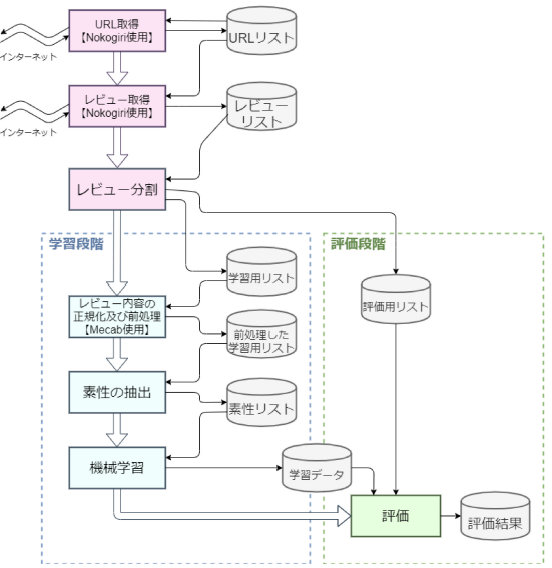
\includegraphics[width=10cm]{images/system1.png}
    \caption{システム概要図}
\end{figure}
この研究はレビューを参考になる順序に並べ替えることが目的のため, 素性には単語の出現頻度を用いている. 
目的変数をレビューが参考になる確率$P$とし, 抽出した素性を用いてロジスティック回帰により学習する. 
ロジスティック回帰のモデル式は式(1)で示される. $\theta_i$は素性の重み, $N$は素性の数を表している. 
\vspace{5truept}

\begin{equation}
    P=\dfrac{1}{1+exp(\theta_0x_0+\theta_1x_1+\cdots+\theta_Nx_N)}
\end{equation}
\vspace{5truept}

次に学習したモデルを用いて, 評価用データに対して実験を行ない, 提案システムの精度を検証している. 
この研究の提案システムの精度の評価は, 実際の商品ページのレビューの並び順との一致率で評価している. 
正解の並び方を$L_R$, 提案システムによる並べ方を$L_P$としたとき, それぞれの要素の一致率を$P_{match}$としている. 
例えば, 以下の並び方のとき, $P_{match}=100\%$となり最も良い結果となる. 
\begin{align}
    L_R:\{1,2,3,4,5\}\notag\\
    L_P:\{1,2,3,4,5\}\notag
\end{align}
しかし, 以下のように並び方の評価としては良い結果と言える場合でも, 5件のレビュー中1件のみ一致していることになり, 
$P_{match}=20\%$と低い結果になる. 
\begin{align}
    L_R:\{1,2,3,4,5\}\notag\\
    L_P:\{4,1,2,3,5\}\notag
\end{align}

このように正しい評価が行えない場合を解決するため, この研究ではクイックソートを利用した新しい評価法のQE法(Quicksort Evaluation method)
を提案している. QE法ではピボットを中央値とし, 昇順にするために要素を入れ替えた回数$S_{count}$と, 要素数における最大の入れ替え回数
$S_{max}$を用いた式(2)により, 評価値$P_{QE}$を求めている. なお, $S_{max}$は全ての要素が逆順の場合にクイックソートで
昇順に入れ替えた回数である. 
\vspace{5truept}

\begin{equation}
    P_{QE}=1-\dfrac{S_{count}}{S_{max}}
\end{equation}
\vspace{5truept}

実際の商品レビュー52,403件を取得し, そのうち51,403件を学習用データ, 1,000件を評価用データに分けて実験を行い, 提案システムの
精度を評価した結果を表1に示している. 
ここで, 登場回数$F$とは学習の素性とするか決定するための単語の出現回数である. 
表1から, $F=5000$, 学習率$\eta=1.7$のときに評価値$P_{QE}=0.814$と最大になる. 従って, この論文で提案しているシステムは
レビューを参考になる順序に並び替える手法として有効であると言える. 

しかし, この論文ではAmazonの商品レビューを分析の対象としていて, 素性には単語の出現頻度を用いているため, 
提案システムが成り立つにはしっかり商品をレビューしている文章を学習させる必要がある. そのため, この論文で提案されているシステム
ではYouTubeで商品を宣伝している動画や, SNSの投稿に対するコメントを学習させた場合に上手く学習できなかったり, 精度が悪くなってしまう
ことが考えられる. なぜならば, YouTubeの動画やSNSの投稿に対するコメントというのは誰でも気軽にでき, 内容も自由であるため, 
商品のレビューのようなコメントの数がAmazonの商品レビューに比べると少ないからである. また, 一文の長さも短いことが多く, 素性となり得る単語の抽出
も難しいと考えられる. そこで, 本論文ではそのような問題を解決するための手法を第Ⅱ部で提案する.
\begin{table}
    \centering
    \caption{登場回数と学習率の組み合わせごとの評価値$P_{QE}$}
    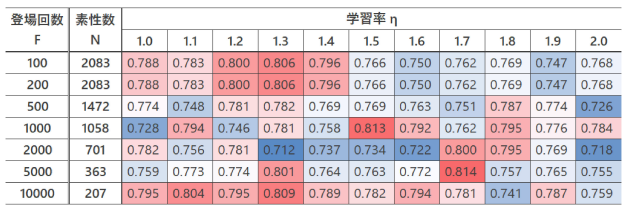
\includegraphics[width=14cm]{images/table1.png}
\end{table}

\subsection{単語の出現頻度と類似性に基づいたトピックモデル洗練化手法[2]}
この論文では, 第Ⅱ部で後述するトピックモデルの一種のLatent Dirichlet Allocation(以下LDA)を自然言語文書に適用する際の
改善案を提案している. 
通常, トピックモデルを自然言語文書に適用する際には, 前処理として分類に不必要なストップワードの除去を行うことが多いが, 
一般的にストップワードリストに含まれている単語を除去するだけでは, 特定の文書にのみ頻出する特徴的な単語
を除去することが出来ず, トピックモデルの精度に影響を及ぼすという問題が存在する. 
また, トピックモデルによって分類したトピックには, 類似したトピックが複数出現し, 
分類の精度が下がるという問題も存在する. 

そこでこの論文では, 前処理として分析対象としている文書から適切なストップワードリストを作成する方法を提案している. 
また, トピックモデルを適用後の後処理として, トピックを構成している単語の類似度からトピック間の距離を算出し, 
類似しているトピックを統合することでより正確なトピック分類を可能にする手法を提案している. 図2は提案手法の全体像である. 
\begin{figure}[h]
    \centering
    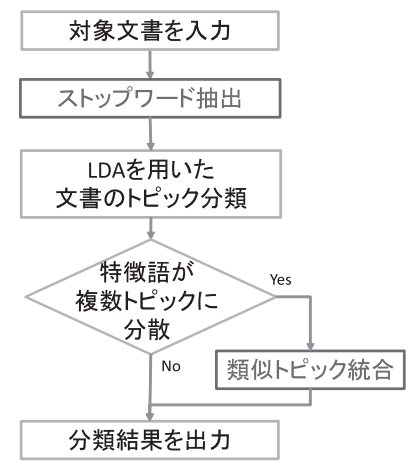
\includegraphics[]{images/fig2.png}
    \caption{提案手法の流れ}
\end{figure}

ストップワードリストを作成する手順を図3で示している. この手法では, まず対象としている文書全体に対して出現率が高い
単語をストップワードとして抽出する. 出現率の算出にははDF(Document Frequency)を用いている. DFとは, 文書全体に対して
ある単語Tが含まれる文書数のことであり, 事前に設定した閾値よりも高いDF値を持つ単語をストップワードリストに加える. 
次に, 抽出した単語と意味的に類似している単語をさらにストップワードとしてリストに加える. 
word2vecを用いて文章中の各単語を周辺の単語から学習し, 単語の分散表現を得て単語間の類似度を算出する.  
それによりある単語Tの類似単語を抽出することができ, ある閾値以上の類似度を示した単語を全てストップワードリストに加える. 
これにより, DF値が高くない場合でも文書の特徴を表しにくい単語をストップワードリストに加えることが可能になる. 
\begin{figure}[h]
    \centering
    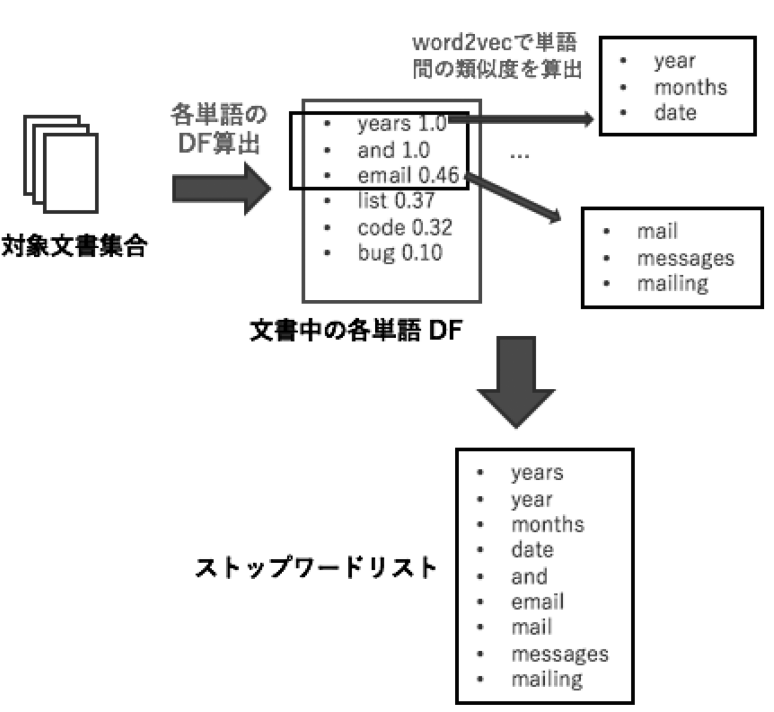
\includegraphics[]{images/fig3.png}
    \caption{ストップワード抽出手法の流れ}
\end{figure}

トピックモデル適用後の後処理では, 分類結果に似たよったトピックが存在する場合にそれらのトピックを統合する処理を行うことを提案している. 
類似トピックの判断基準には, TF-IDF cos類似度推定法が用いられている. これは, cos類似度の計算に使用する
ベクトルの成分をTF-IDFで算出したものにした手法である. この研究では, 分類した各トピックの単語集合に対して
TF-IDF cos類似度を利用したクラスタリングを行い, その結果に従ってトピックを統合する手法を提案している. 

以上の提案手法をLDAのよるメーリングリストのトピック分類に適用し, 評価項目に基づいて比較することで提案手法
の有効性の評価を行っている. 評価項目として, 一般的なストップワードリストを用いた手法と提案手法を比較している. 
また, 後処理として類似トピックの統合を行った場合についても比較を行っている. 
トピック分類の正確さを評価する指標として, 適合率, 再現率, それらの調和平均のF値を採用している. 
実験結果を表2に示している. 
\begin{table}
    \centering
    \caption{ストップワード数($\#N$), 適合率, 再現率, F値の結果}
    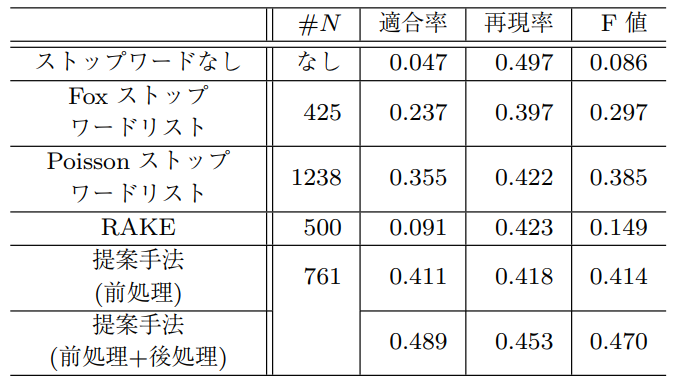
\includegraphics[]{images/table2.png}
\end{table}



\newpage
\section{研究目的}
研究目的

\newpage
\part{提案手法}
\section{トピックモデル}
トピックモデルの説明
\subsection{Latent Dirichlet Allocation}
LDAの説明
\subsection{Biterm Topic Model}
BTMの説明
\newpage
\section{提案システム}
ここでは, 前項で説明したBitem Topic Modelを用いて, YouTube上で自社製品やサービスを宣伝している動画
に対するユーザーのコメントから, 宣伝している商品やサービスに対して関連性が高いコメントを抽出する
システムを提案する. また, 提案したシステムの精度を検証する方法についても説明する. 
\subsection{データ収集}
実験に用いるYouTubeのコメントは, YouTube Data API v3を用いて取得した. 
\subsection{前処理手法}
\subsection{BTMによるトピック抽出}
\subsection{文章生成}
\subsection{文章間の類似度計算}
\subsection{提案システムの精度検証}
\newpage
\part{実験結果}
\section{実験目的、仮説}
\part{参考文献}
[1]機械学習を用いた自然言語処理による商品レビューの評価

[2]単語の出現頻度と類似性に基づいたトピックモデル洗練化手法
\end{document}